% ============================================================================
% Chapitre 4 : Réalisation
% ============================================================================
\chapter{Réalisation du prototype}
\label{chap:realisation}

\introchap

Ce chapitre décrit comment la conception a été réalisée. Il présente l'organisation du dépôt, le serveur et ses routes, la base de données et l'authentification, les canaux temps réel, les interfaces du patient et du médecin, la visioconsultation côté navigateur, puis l'installation et le déploiement. Les extraits de code sont ceux du dépôt.

\section{Organisation du dépôt}

\begin{lstlisting}[language={}, numbers=none, caption={Arborescence du dépôt.}]
app/       main.py       FastAPI : routes REST, WebSocket, sécurité
           auth.py       connexion, sessions, jetons
           database.py   schéma SQLite, hachage des mots de passe
static/    index.html, styles.css
           app.js        interfaces patient et médecin, graphiques, WebRTC
tests/     test_api.py   37 tests automatisés
scripts/   benchmark.py  mesures chiffrées
           smoke_test.py parcours complet contre n'importe quelle adresse
           sus_score.py  calcul du score d'utilisabilité
docs/      architecture, BPMN, sécurité, validation, rapport/
\end{lstlisting}

L'application se lance par une seule commande (\code{uvicorn app.main:app}) et s'ouvre à l'adresse \code{http://127.0.0.1:8000}. Le serveur sert aussi les fichiers de l'interface~: aucun serveur web séparé n'est nécessaire.

\section{Le serveur FastAPI}

\subsection{Validation des données}

Les règles de validation sont déclarées une seule fois, dans des classes Pydantic. Une valeur hors bornes est refusée par le framework avec le code HTTP~422, avant même d'atteindre la base.

\begin{lstlisting}[language=Python, caption={Validation d'une mesure (extrait de \code{app/main.py}).}, label=lst:validation]
class VitalInput(BaseModel):
    systolic: int = Field(ge=70, le=250)
    diastolic: int = Field(ge=40, le=160)
    heart_rate: int = Field(ge=30, le=220)
    spo2: int = Field(ge=70, le=100)
    temperature: float = Field(ge=32, le=43)
\end{lstlisting}

\subsection{Règles d'alerte}

La fonction \code{alert\_for} compare une mesure validée aux seuils du tableau~\ref{tab:seuils}. Elle retourne au plus une alerte, qui regroupe tous les dépassements et dont la gravité est critique dès qu'un problème l'est.

\begin{lstlisting}[language=Python, caption={Règles d'alerte (\code{alert\_for}).}, label=lst:alert]
def alert_for(vital: VitalInput):
    issues = []
    if vital.systolic >= 180 or vital.diastolic >= 120:
        issues.append("Tension artérielle critique")
    if vital.spo2 < 90:
        issues.append("Saturation en oxygène critique")
    if vital.heart_rate < 45 or vital.heart_rate > 130:
        issues.append("Fréquence cardiaque hors seuil")
    if vital.temperature >= 39.0:
        issues.append("Fièvre élevée")
    if not issues:
        return None
    severity = "critical" if any("critique" in i for i in issues) else "warning"
    return severity, " · ".join(issues)
\end{lstlisting}

\subsection{Contrôle d'accès}

Chaque route appelle l'une de trois petites fonctions. L'interface masque certains menus pour le confort, mais c'est le serveur qui décide réellement.

\begin{lstlisting}[language=Python, caption={Contrôle de la session et des rôles.}, label=lst:roles]
def current_user(request: Request) -> dict:
    user = user_for_token(bearer_token(request))
    if not user:
        raise HTTPException(401, "Session absente ou expirée. Veuillez vous reconnecter.")
    return user

def doctor_only(user: dict = Depends(current_user)) -> dict:
    if user["role"] != "doctor":
        raise HTTPException(403, "Action réservée au médecin.")
    return user

def ensure_patient_access(user: dict, patient_id: int) -> None:
    if user["role"] == "patient" and user["patient_id"] != patient_id:
        raise HTTPException(403, "Accès refusé à ce dossier patient.")
\end{lstlisting}

\subsection{Envoi d'une mesure}

La route d'envoi d'une mesure enchaîne vérification des droits, validation, enregistrement et comparaison aux seuils. Selon le résultat, le médecin reçoit un événement \code{alert} ou un événement \code{vital}, de façon asynchrone, sans retarder la réponse au patient.

\section{Base de données et authentification}

La base est un fichier SQLite accédé par une seule fonction de connexion, qui ouvre, valide puis ferme. Les requêtes sont toutes paramétrées, ce qui rend l'injection \ac{SQL} impossible. Les mots de passe ne sont jamais conservés en clair~: ils sont transformés par \ac{PBKDF2} avec \ac{SHA}-256, 200\,000 itérations et un sel aléatoire propre à chaque compte~\cite{rfc8018}.

\begin{lstlisting}[language=Python, caption={Hachage et vérification des mots de passe (\code{app/database.py}).}, label=lst:hash]
PBKDF2_ITERATIONS = 200_000

def hash_password(password: str, salt_hex: str):
    return hashlib.pbkdf2_hmac(
        "sha256", password.encode(), bytes.fromhex(salt_hex), PBKDF2_ITERATIONS
    ).hex()

def verify_password(password: str, salt_hex: str, expected_hex: str) -> bool:
    return hmac.compare_digest(hash_password(password, salt_hex), expected_hex)
\end{lstlisting}

À la connexion, le serveur génère un jeton aléatoire de 32~octets et ne conserve en base que son empreinte \ac{SHA}-256, avec une validité de 8~heures. Une fuite de la base ne donne donc aucune connexion exploitable. Comme le hachage est volontairement lent, il s'exécute dans un fil séparé pour ne pas bloquer les autres requêtes.

\section{Canaux temps réel}

Deux \ac{WS} sont ouverts par le navigateur. Le premier message de chaque connexion doit être \code{\{"type": "auth", "token": ...\}}~: sans jeton valide, le serveur répond \code{auth-failed} et ferme la connexion. L'origine de la page est contrôlée, y compris derrière un proxy, pour bloquer le détournement de WebSocket depuis un autre site. La signalisation vérifie en plus que l'utilisateur est le médecin ou le patient de la consultation ouverte (sinon \code{forbidden}) et limite la salle à deux participants (sinon \code{room-full}). Quand l'un des deux quitte la salle, l'autre reçoit un message \code{leave} et peut attendre son retour.

\section{Interfaces utilisateur}

L'interface est en français et fonctionne sur ordinateur et sur mobile. Elle propose un écran de connexion avec deux comptes de démonstration, un formulaire d'inscription validé côté client et côté serveur, un espace patient et un espace médecin.

\begin{figure}[htbp]
\centering
\begin{subfigure}[t]{0.38\textwidth}
  \centering
  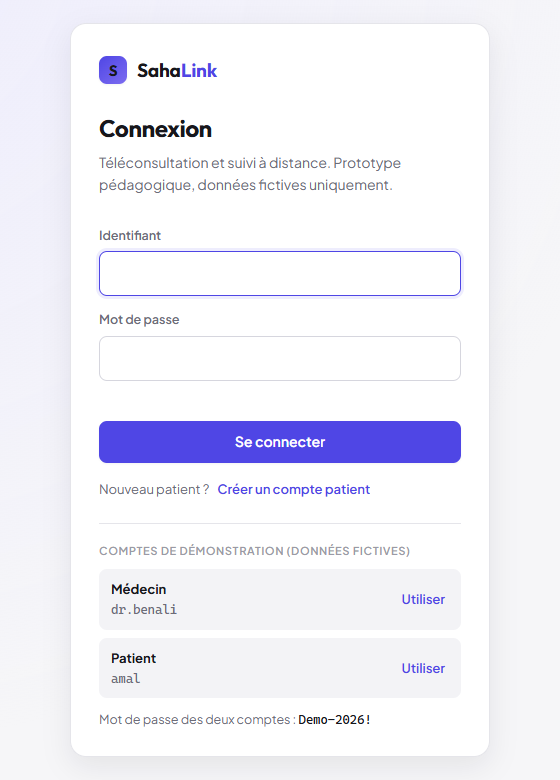
\includegraphics[width=\textwidth]{images/screenshots/connexion_crop.png}
  \caption{Connexion.}
\end{subfigure}\hfill
\begin{subfigure}[t]{0.38\textwidth}
  \centering
  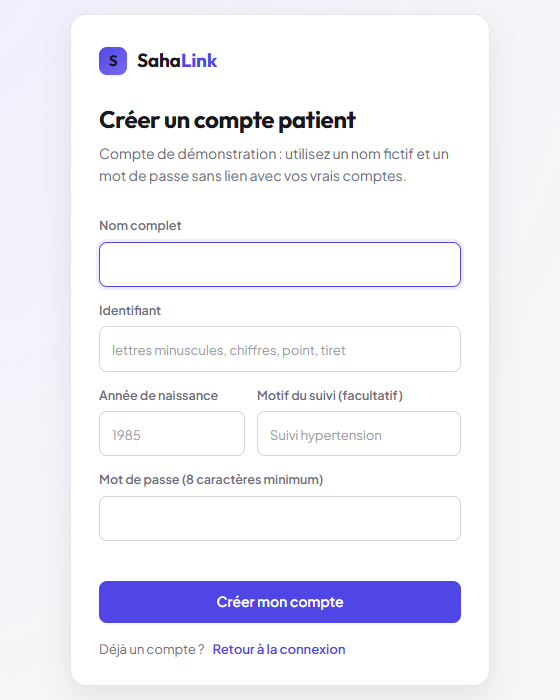
\includegraphics[width=\textwidth]{images/screenshots/inscription_crop.png}
  \caption{Inscription d'un patient.}
\end{subfigure}
\caption{Écrans d'accès (données fictives).}
\label{fig:acces}
\end{figure}

\subsection{Espace patient}

Le patient donne ou retire son consentement (case à cocher et bouton), saisit ses cinq constantes, peut préremplir des valeurs dangereuses avec le bouton \enquote{Simuler une alerte} (utile à la démonstration), consulte son historique et rejoint la consultation lorsqu'il est invité.

\begin{figure}[htbp]
\centering
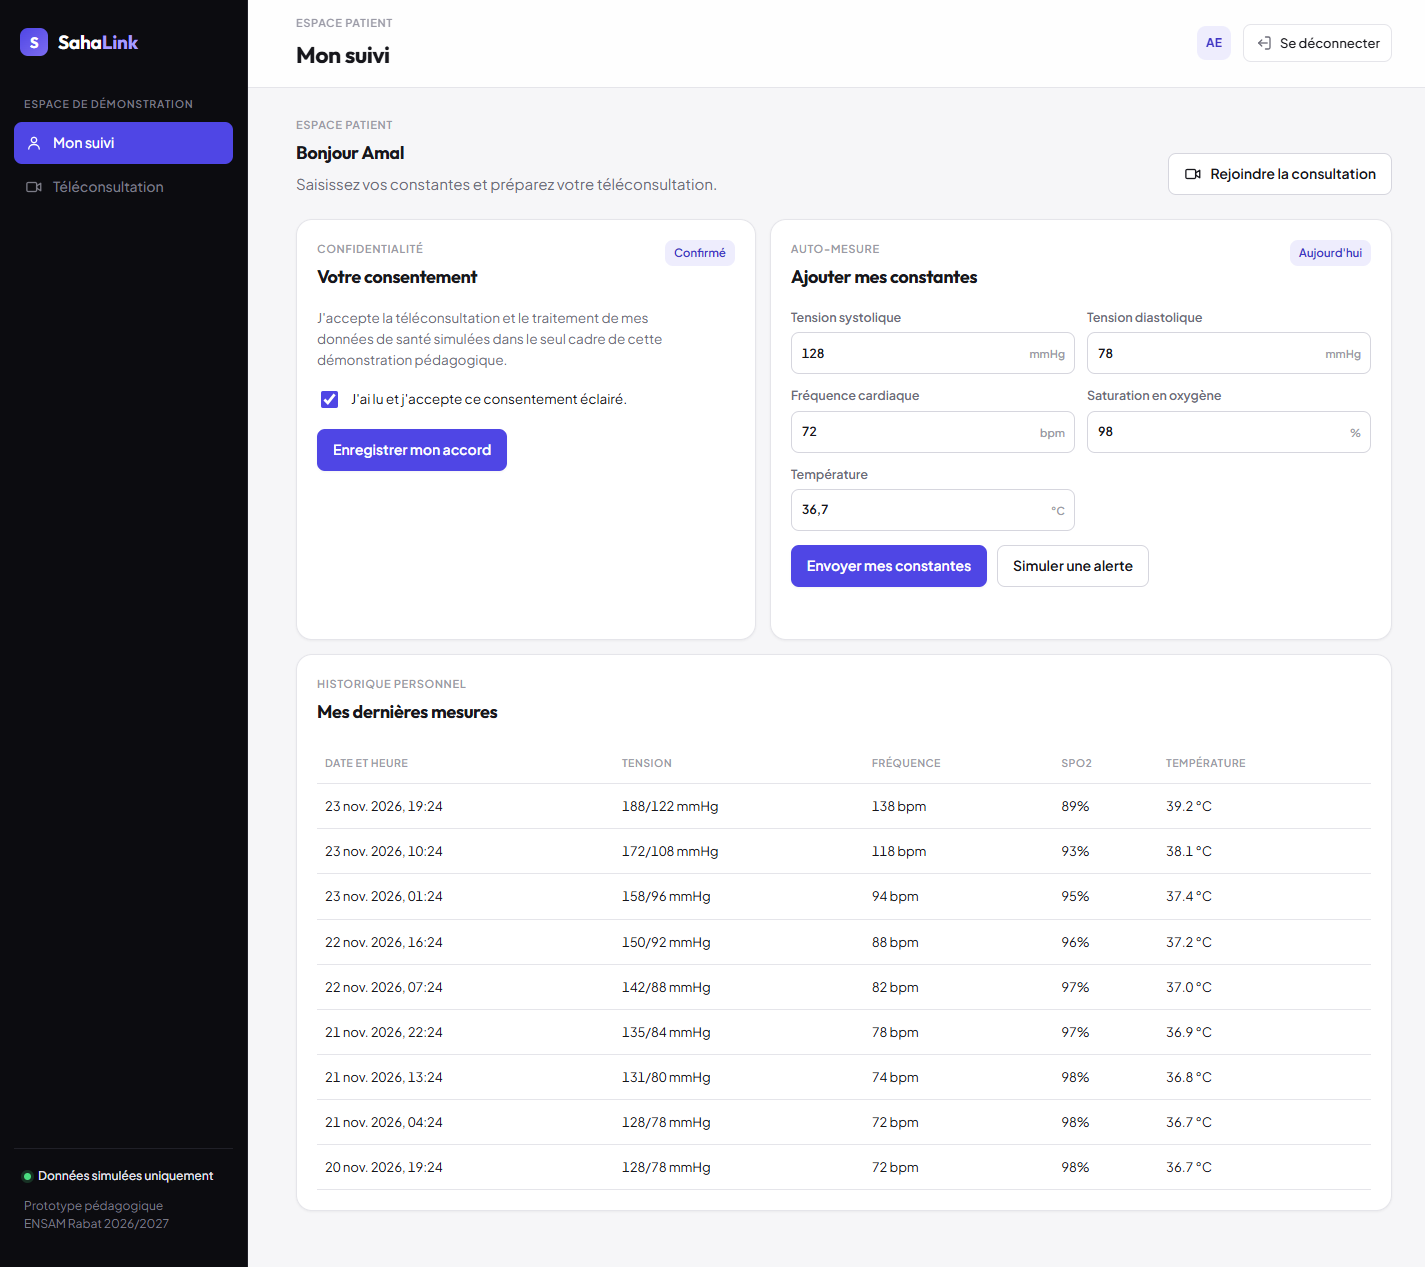
\includegraphics[width=0.46\textwidth]{images/screenshots/patient.png}
\caption{Espace patient~: consentement, saisie des constantes et historique personnel.}
\label{fig:patient}
\end{figure}

\subsection{Espace médecin}

Le médecin voit le nombre de patients suivis et d'alertes ouvertes, choisit un patient dans une liste qui indique pour chacun les alertes ouvertes et l'état du consentement, lit les valeurs courantes, reçoit les alertes en temps réel et peut les acquitter. Quatre petits graphiques en SVG intégré (tension, fréquence cardiaque, \ac{SpO2}, température) montrent l'évolution des mesures avec des lignes de seuil~: les points rouges signalent une valeur critique et les points orange une valeur à surveiller.

\begin{figure}[htbp]
\centering
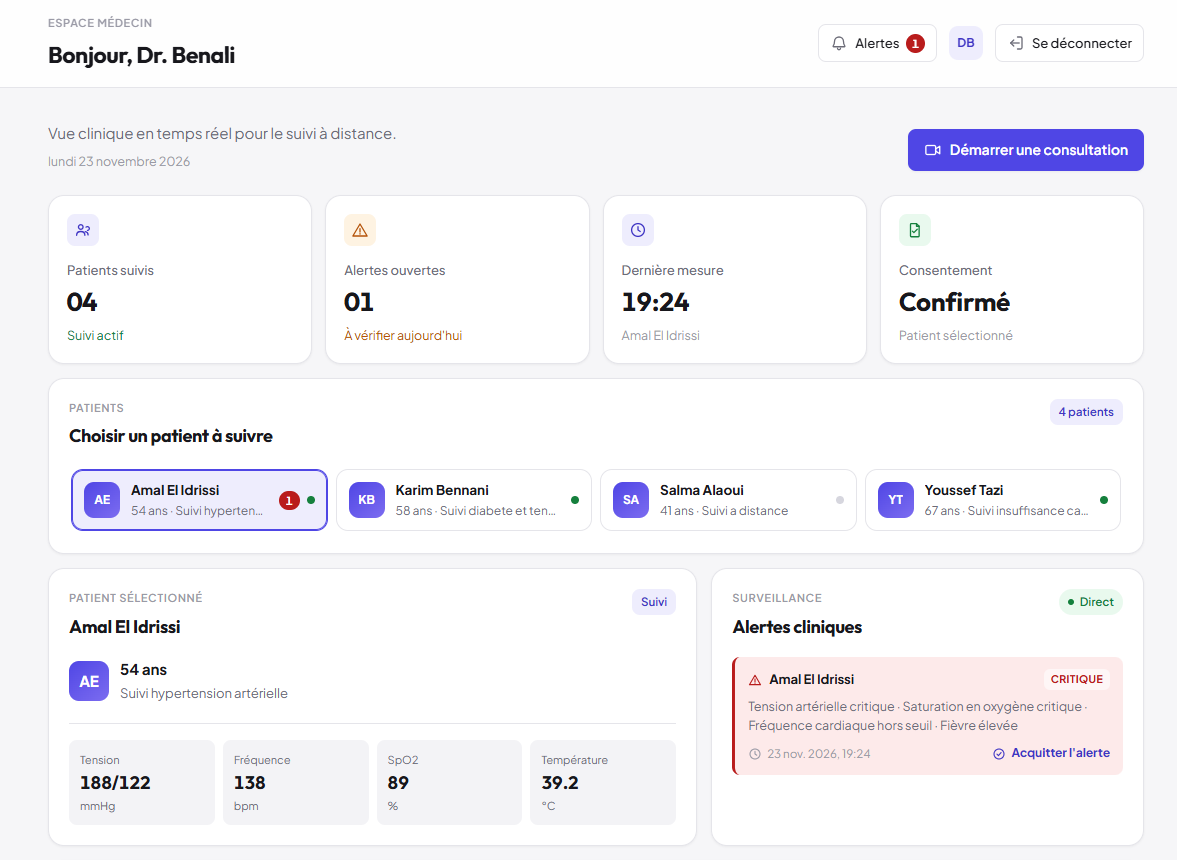
\includegraphics[width=0.74\textwidth]{images/screenshots/medecin_haut.png}
\caption{Espace médecin~: liste des patients, alerte critique et valeurs courantes (données fictives).}
\label{fig:medecin}
\end{figure}

\begin{figure}[htbp]
\centering
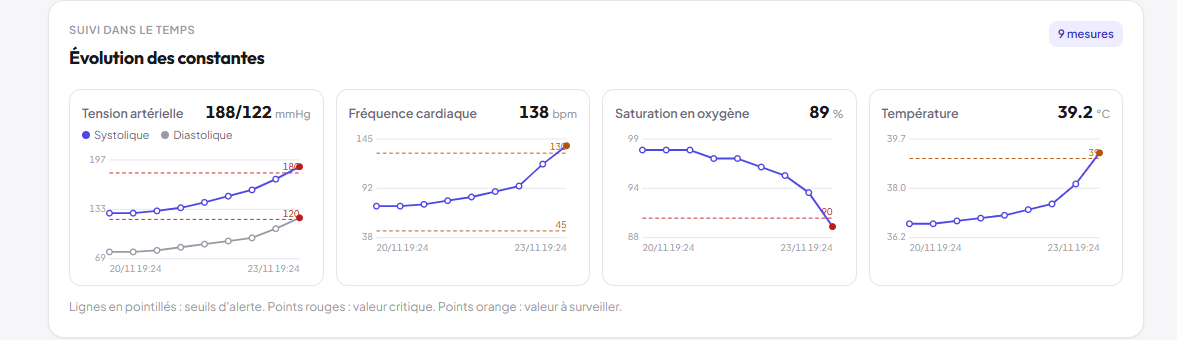
\includegraphics[width=0.74\textwidth]{images/screenshots/medecin_graphiques.png}
\caption{Évolution des quatre constantes avec lignes de seuil (pointillés) et points d'alerte.}
\label{fig:graphiques}
\end{figure}

\section{Visioconsultation côté navigateur}

La vidéo est gérée par le code JavaScript de \code{static/app.js}, qui crée une connexion \code{RTCPeerConnection} par appel. Quatre points méritent d'être signalés.

\begin{itemize}
  \item \textbf{Négociation sans blocage}~: le code applique le motif des pairs \enquote{polis}. Si les deux navigateurs envoient une offre en même temps, l'un abandonne la sienne pour accepter celle de l'autre.
  \item \textbf{Choix de la caméra}~: les caméras virtuelles de téléphone (Camo, Iriun) sont classées en dernier, et chaque candidate est testée sur une image réelle (mesure de la luminosité) avant d'être retenue. Une liste permet de changer de caméra en cours d'appel sans renégocier.
  \item \textbf{Diagnostic explicite}~: si la caméra renvoie une image noire, le statut dit si le problème vient de la caméra locale ou de celle de l'interlocuteur.
  \item \textbf{Serveurs de traversée}~: la configuration \ac{ICE} est servie par la route \code{/api/rtc-config}. Par défaut, des serveurs \ac{STUN} publics sont utilisés~; un relais \ac{TURN} peut être ajouté par la variable d'environnement \code{ICE\_SERVERS} pour les réseaux stricts.
\end{itemize}

La capture réelle de la caméra et du micro ne peut pas être automatisée~: elle est validée manuellement sur deux navigateurs (chapitre~\ref{chap:validation}).

\section{Installation et déploiement}

Trois variables d'environnement règlent le comportement~: \code{SAHALINK\_DB\_PATH} (fichier SQLite, utilisé par les tests pour une base temporaire), \code{ICE\_SERVERS} (liste \ac{JSON} de serveurs \ac{STUN} ou \ac{TURN}) et \code{SAHALINK\_FORCE\_HTTPS} (redirection vers HTTPS). Pour une démonstration entre deux ordinateurs, la caméra exige un contexte sécurisé~: le serveur local est exposé par un tunnel \ac{HTTPS} (Cloudflare), qui fournit aussi le chiffrement du transport. Un \code{Procfile} et un plan de déploiement sont fournis pour un hébergement qui accepte un serveur de longue durée (les \ac{WS} excluent les plateformes sans serveur). La procédure complète figure en annexe~\ref{ann:installation}.

\conclchap

La réalisation tient en trois fichiers Python et un fichier JavaScript. Les règles du chapitre~\ref{chap:cadrage} sont déclarées une seule fois (Pydantic, \code{alert\_for}, fonctions de contrôle), la sécurité des secrets est intégrée au schéma (sel, empreinte du jeton), et les deux interfaces affichent les mêmes données avec des droits différents. Le chapitre suivant évalue ce prototype par un scénario clinique complet, des tests automatiques et des mesures chiffrées.
